% ---------------------------------------------------------------------------
% Author guideline and sample document for EG publication using LaTeX2e input
% D.Fellner, v1.13, Jul 31, 2008

\documentclass{egpubl}
\usepackage{eg2015}

% --- for  Annual CONFERENCE
%\ConferenceSubmission   % uncomment for Conference submission
\ConferencePaper        % uncomment for (final) Conference Paper
% \STAR                   % uncomment for STAR contribution
% \Tutorial               % uncomment for Tutorial contribution
% \ShortPresentation      % uncomment for (final) Short Conference Presentation
% \Areas                  % uncomment for Areas contribution
% \MedicalPrize           % uncomment for Medical Prize contribution
% \Education              % uncomment for Education contribution
%
% --- for  CGF Journal
% \JournalSubmission    % uncomment for submission to Computer Graphics Forum
% \JournalPaper         % uncomment for final version of Journal Paper
%
% --- for  CGF Journal: special issue
% \SpecialIssueSubmission    % uncomment for submission to Computer Graphics Forum, special issue
% \SpecialIssuePaper         % uncomment for final version of Journal Paper, special issue
%
% --- for  EG Workshop Proceedings
% \WsSubmission    % uncomment for submission to EG Workshop
% \WsPaper         % uncomment for final version of EG Workshop contribution
%
 \electronicVersion % can be used both for the printed and electronic version

% !! *please* don't change anything above
% !! unless you REALLY know what you are doing
% ------------------------------------------------------------------------

% for including postscript figures
% mind: package option 'draft' will replace PS figure by a filname within a frame
%\ifpdf \usepackage[pdftex]{graphicx} \pdfcompresslevel=9
%\else \usepackage[dvips]{graphicx} \fi

\PrintedOrElectronic

% prepare for electronic version of your document
\usepackage{t1enc,dfadobe}

\usepackage{egweblnk}
\usepackage{cite}
\usepackage{balance}

% For backwards compatibility to old LaTeX type font selection.
% Uncomment if your document adheres to LaTeX2e recommendations.
% \let\rm=\rmfamily    \let\sf=\sffamily    \let\tt=\ttfamily
% \let\it=\itshape     \let\sl=\slshape     \let\sc=\scshape
% \let\bf=\bfseries

% end of prologue

%\input{EGauthorGuidelines-body.inc}
% ---------------------------------------------------------------------
% EG author guidelines plus sample file for EG publication using LaTeX2e input
% D.Fellner, v1.17, Sep 23, 2010


\title[PGVD]%
      {An Adaptive, Parallel Algorithm for Approximating the Generalized Voronoi Diagram}

% for anonymous conference submission please enter your SUBMISSION ID
% instead of the author's name (and leave the affiliation blank) !!
% For Computer Graphics Forum: Please use the abbreviation of your first name.

%% author example
%\author[D. Fellner \& S. Behnke]
%       {D.\,W. Fellner\thanks{Chairman Eurographics Publications Board}$^{1,2}$
%        and S. Behnke$^{2}$
%        S. Spencer$^2$\thanks{Chairman Siggraph Publications Board} \\
%         $^1$TU Darmstadt \& Fraunhofer IGD, Germany \\
%         $^2$Institut f{\"u}r ComputerGraphik \& Wissensvisualisierung, TU Graz, Austria
%       }

\author[J. Edwards \& N. Vollmer \& N. Harrison]
%       {John Edwards\thanks{jedwards@sci.utah.edu}$^1$ and
%       {John Edwards\\
       {John Edwards and
         Nathan Vollmer and
         Nicholas Harrison \\
         \parbox[t]{10cm}{\centering Idaho State University}
%         $^2$Google, Inc. \\
%         \footnotesize{$^3$The University of Texas at Austin}}
       }
%\author[paper1040]
%       {paper1040}

% ------------------------------------------------------------------------

% if the Editors-in-Chief have given you the data, you may uncomment
% the following five lines and insert it here
%
% \volume{27}   % the volume in which the issue will be published;
% \issue{1}     % the issue number of the publication
% \pStartPage{1}      % set starting page

\renewcommand{\paragraph}[1]{\noindent \textbf{#1}}
%\usepackage{amsmath,amsthm,amsfonts,amscd,amssymb,amstext} 
\usepackage{amsmath,amsfonts,amscd,amssymb,amstext} 
\usepackage{mathrsfs}
				% Some packages to write mathematics.
\usepackage{overpic}
\usepackage{eucal} 	 	% Euler fonts
\usepackage{verbatim}      	% Allows quoting source with commands.
\usepackage{makeidx}       	% Package to make an index.
%\usepackage{citesort}         	% 
\usepackage{subfig}
\usepackage{graphicx}
\usepackage{url}		% Allows good typesetting of web URLs.
\usepackage{multirow}
%\usepackage[linesnumbered, noline]{algorithm2e}
%\usepackage[boxed, noline]{algorithm2e}
\usepackage[ruled]{algorithm2e}
\usepackage{booktabs}
\usepackage{tabularx}
\usepackage{array}
\usepackage{adjustbox}
\usepackage{color}
\usepackage{tikz}
% To balance the columns at the end
\usepackage{balance}
\usepackage[mediumspace,mediumqspace,Grey,squaren]{SIunits}
%\usepackage{draftcopy}		% Uncomment this line to have the
				% word, "DRAFT," as a background
				% "watermark" on all of the pages of
				% of your draft versions. When ready
				% to generate your final copy, re-comment
				% it out with a percent sign to remove
				% the word draft before you re-run
				% Makediss for the last time.
\usepackage[normalem]{ulem}

%\usepackage{cite}
\usepackage{balance}
\usepackage{color}

\definecolor{bostonuniversityred}{rgb}{0.8, 0.0, 0.0}
\definecolor{medblue}{rgb}{0.0, 0.0, 0.7}

%------------------------------------------------------------
% Custom commands
%------------------------------------------------------------
%\newcommand{\old}[1]{\textcolor{blue}{\sout{#1}}}
\newcommand{\old}[1]{}

%\newcommand{\red}[1]{\textcolor{red}{#1}}
\newcommand{\red}[1]{\textcolor{bostonuniversityred}{#1}}
\newcommand{\blue}[1]{\textcolor{medblue}{#1}}
\definecolor{light-gray}{gray}{0.75}
\newcommand{\gray}[1]{\textcolor{light-gray}{#1}}
%\newcommand{\red}[1]{#1}

%\newcommand{\reconstruct}{RECONSTRUCT\textsuperscript{\texttrademark}}
%\newcommand{\tm}{\textsuperscript{\texttrademark}}
\newcommand{\tm}{$^1$}
\newcommand{\addref}{\red{REF}}
\newcommand{\mathtext}[1]{\text{#1}}
\newcommand{\etal}{et al.\ }
\newcommand{\algorithmspace}{\vspace{8pt}}
\newcommand{\glfs}{\emph{glfs}}

\renewcommand{\vec}[1]{\mathbf{#1}}

\newcommand{\centercell}[1]{\multicolumn{1}{c}{#1}}
\newcolumntype{x}[1]{>{\centering\arraybackslash\hspace{0pt}}m{#1}}
\newcolumntype{y}[1]{>{\centering\arraybackslash\hspace{0pt}}m{#1\textwidth}}
\newcolumntype{M}{>{\centering\arraybackslash}m{1cm}}

\DeclareMathOperator*{\argmin}{arg\,min}
\DeclareMathOperator*{\argmax}{arg\,max}

\newcommand{\BigO}[1]{\ensuremath{\operatorname{O}\left(#1\right)}}
\newcommand{\centroid}{\mathscr{C}}
\newcommand{\iring}{\mathscr{R}}

% aligned
\renewcommand{\d}{\delta}
\newcommand{\vempty}{\mathscr{E}}
\newcommand{\e}{\epsilon}
\newcommand{\dist}{\mathtext{dist}}
\newcommand{\ball}{\mathscr{B}}


\newcommand{\hgt}{22mm}

%%--------------------------------------------------
%% Theorem environments (amsthm package required)
%%--------------------------------------------------
%% \theoremstyle{plain} %% This is the default
%\newtheorem{theorem}{Theorem}
%\newtheorem{lemma}{Lemma}
%\newtheorem{corollary}{Corollary}
%\newtheorem{conjecture}{Conjecture}
%\newtheorem{crit}{Criterion}
%\newtheorem{condition}{Condition}
%\newtheorem{fact}{Fact}

%\theoremstyle{definition}
%\newtheorem{defn}{Definition}[section]

%\theoremstyle{remark}
%\newtheorem{rem}{Remark}[section]
%\newtheorem*{notation}{Notation}

%\numberwithin{equation}{section}

%--------------------------------------------------
% Tight enumerations
%--------------------------------------------------
\newenvironment{tightenumerate}{
\begin{enumerate}
  \setlength{\itemsep}{1pt}
  \setlength{\parskip}{0pt}
  \setlength{\parsep}{0pt}
}{\end{enumerate}
}
\newenvironment{tightitemize}{
\begin{itemize}
  \setlength{\itemsep}{1pt}
  \setlength{\parskip}{0pt}
  \setlength{\parsep}{0pt}
}{\end{itemize}
}

%--------------------------------------------------
% Add figs to graphics path
%--------------------------------------------------
\graphicspath{{./}{./figs/}}

\newcolumntype{H}{@{}>{\lrbox0}l<{\endlrbox}}

%\newcommand{\container}[2]{container(#1, #2)}
\newcommand{\container}[1]{container(#1)}

\newcommand{\directAncestors}[1]{direct\_ancestors(#1)}

\newcommand{\lcp}{\textit{lcp}}

\newcommand{\shortcite}[1]{\cite{#1}}

\renewcommand{\paragraph}[1]{\noindent \textbf{#1}}



%-------------------------------------------------------------------------
\begin{document}

%\teaser{
%  \subfloat[][]{
%    \label{fig:gears1}
%    \begin{tikzpicture}
%      \node[anchor=south west,inner sep=0] at (0,0) {
%        \begin{tabular}[b]{c}
%          \includegraphics[height=0.8in]{gears-far1.png} \\
%          \includegraphics[height=0.8in]{gears-close1.png}
%        \end{tabular}
%      };
%      \draw[black,thick] (1.4,3.2) rectangle (2.0,3.6);
%      \draw[black,dashed] (1.4,3.6) -- (0.22,2.15);
%      \draw[black,dashed] (2.0,3.6) -- (2.95,2.15);
%      \draw[black,thick] (0.22,0.1) rectangle (2.95,2.15);
%    \end{tikzpicture}
%  }
%  \subfloat[][]{
%    \label{fig:gears}
%    \begin{tikzpicture}
%      \node[anchor=south west,inner sep=0] at (0,0) {
%        \begin{tabular}[b]{c}
%          \includegraphics[height=0.8in]{gears-far4.png} \\
%          \includegraphics[height=0.8in]{gears-close4.png}
%        \end{tabular}
%      };
%      \draw[black,thick] (1.3,3.1) rectangle (1.9,3.5);
%      \draw[black,dashed] (1.3,3.5) -- (0.22,2.15);
%      \draw[black,dashed] (1.9,3.5) -- (2.92,2.15);
%      \draw[black,thick] (0.22,0.1) rectangle (2.92,2.15);
%    \end{tikzpicture}
%  }
%  \hspace{3mm}
%  \subfloat[][]{
%    \label{fig:knife}
%    \includegraphics[trim=4cm 0cm 4cm 2.5cm, clip=true, height=1.4in]
%                    {knife-above/slice-00000.png}
%  }
%  \subfloat[][]{
%    \label{fig:knife2}
%    \includegraphics[trim=2mm 0cm 2mm 2cm, clip=true, height=1.4in]
%                    {knife-above/slice-00110.png}
%  }
%  \caption{Two example applications of the \red{approximated} generalized Voronoi diagram (GVD) computed by our novel, adaptive algorithm. Previous GVD methods require a gridded space of $2^{24}$ (gears dataset) and $2^{36}$ (knives dataset) voxels to resolve the closely spaced objects.
%    \protect\subref{fig:gears1} Two gears with regions of very tight spacing.
%    \protect\subref{fig:gears} The GVD of the gears model.  The surface is colored red in areas of very close tolerance.
%    \protect\subref{fig:knife} Three butter knives in a wood block.  To animate removal of the knives without intersecting the block requires extreme care because of close mesh spacing.
%    \protect\subref{fig:knife2} Intersection-free motion is guaranteed by computing motion vectors based on the GVD and allowing motion only within a Voronoi cell.
%  }
%  \label{fig:teaser}
%}
%
\maketitle

\begin{abstract}
We present a parallel algorithm that approximates the Generalized Voronoi Diagram (GVD) on arbitrary collections of 2D or 3D geometric objects. Our algorithm is hierarchical, not uniformly gridded, enabling us to compute the GVD on datasets with extremely close object tolerances, including intersections. We demonstrate our method on a variety of data and show example applications of the GVD in 2D and 3D. \\

%   Leave one blank line after the abstract, 
%   then add the subject categories according to the ACM Classification Index 
%   (see http://www.acm.org/class/1998/).

\begin{classification} % according to http://www.acm.org/class/1998/
  \CCScat{I.3.5}{Computer Graphics}{Computational Geometry and Object Modeling}{Boundary representations}
  \CCScat{I.3.6}{Computer Graphics}{Methodology and Techniques}{Graphics data structures and data types}
  %\CCScat{Computer Graphics}{I.3.3}{Picture/Image Generation}{Line and curve generation}
\end{classification}

\end{abstract}

%-------------------------------------------------------------------------
% Body
%-------------------------------------------------------------------------

%-------------------------------------------------------------------------------
% introduction
%-------------------------------------------------------------------------------
\section{Introduction}
\label{sec:intro}
Previous paper: \cite{edwards2015approximating}

\red{The generalized Voronoi diagram (GVD) is an important structure that divides space into a complex of generalized Voronoi cells (GVCs) around objects.  Similar to the ordinary Voronoi diagram, each GVC contains exactly one object, or site, and every point in the GVC is closer to its contained object than to any other object.  The generalized Voronoi diagram is the boundary of the cell complex, and thus every point on the GVD is equidistant from two or more closest objects.  Applications of the GVD range from motion path planning to GIS analysis to mosaicking.

Ordinary Voronoi diagrams have been studied extensively and efficient algorithms exist to compute them, but the GVD is difficult to compute analytically in general \cite{boissonnat2006curved,hoff1999fast} and so the majority of approaches compute an approximation.  Whereas most algorithms are efficient and robust on certain datasets, all algorithms to our knowledge require inordinate amounts of memory on datasets where objects are very closely spaced relative to the size of the domain.  The failures occur because the space is uniformly gridded.  In such approaches, voxel size must be small enough to resolve object spacings, and if two objects are very close to each other the number of voxels can become prohibitively large.

We present an algorithm to compute a GVD approximation on arbitrary datasets, including those with closely spaced objects.  The approach applies a distance transform over an octree representation of the objects.  Our octree, its associated data structure, and our distance transform are novel and optimized to GVD \red{approximation. For the remainder of the paper, ``GVD'' will refer to the approximated Generalized Voronoi Diagram.}

This paper demonstrates GVD computation on data beyond the computational abilities of previous algorithms, unlocking interesting and important applications.  Our approach allows GVD-based proximity queries and other applications using a larger class of meaningful datasets.
}

\paragraph{Main contributions} The primary technical contributions described in the paper are as follows.

\begin{enumerate}
\item Contribution 1
\item Contribution 2
\item Contribution 3
\end{enumerate}

We demonstrate various applications of the GVD...

Our GVD algorithm has a few main steps: 1) ...

%-------------------------------------------------------------------------------
% Related work
%-------------------------------------------------------------------------------
\section{Related work}
Related work falls into two categories: algorithms that compute the GVD and algorithms that compute distance fields, many of which are adaptive.

\paragraph{Generalized Voronoi diagrams}
A theoretical framework for generalized Voronoi diagrams can be found in Boissonnat \etal \shortcite{boissonnat2006curved}. Ordinary Voronoi diagrams are well studied and efficient algorithms exist that compute them exactly \cite{de2008computational}, but exact algorithms for the generalized Voronoi diagram are limited to a small set of special cases \cite{lee1982medial,karavelas2004robust}. In an early work, Lavender \etal \shortcite{lavender1992voronoi} define and compute GVDs over a set of solid models using an octree.  Etzion and Rappoport \shortcite{etzion2002computing} represent the GVD bisector symbolically for lazy evaluation, but are limited to sites that are polyhedra.  Boada \etal \shortcite{boada2002voronoi,boada2008approximations} use an adaptive approach to GVD computation, but their algorithm is restricted to GVDs with connected regions and is inefficient for polyhedral objects with many facets.  Two other works are adaptive \cite{teichmann1997polygonal,vleugels1998approximating} but are computationally expensive and are restricted to convex sites.

In recent years Voronoi diagram algorithms that take advantage of fast graphics hardware have become more common \cite{cao2010parallel,fischer2006fast,hsieh2005simple,rong2007variants,sud2006interactive,sud2006fast,hoff1999fast,wu2008gpu}.  These algorithms are efficient and generalize well to the GVD, but most are limited to a subset of site types.  More importantly, all of them use uniform grids and require an extraordinary number of voxels to resolve closely spaced objects (for example, Figs. \ref{fig:knife} and \ref{fig:path} would require $2^{36}$ and $2^{48}$ voxels, respectively).  To our knowledge, ours is the first fully adaptive algorithm that computes the generalized Voronoi diagram for arbitrary datasets.

\paragraph{Distance fields and octrees}
The GVD is a subset of the locus of distance field critical points, a property that we take advantage of. In that light, the GVD could be a post-processing step to any method that computes a distance field.  Distance transforms compute a distance field, but most are uniformly gridded \cite{jones20063d} and are thus no more suitable than GVD algorithms that use the GPU.

% JME: note that in the Bastos work, ``reconstruction'' is reconstruction
% of the surface from the octree at rendering time.
Two seminal works adaptively compute the Adaptive Distance Field (ADF) on octree vertices.  Strain~\shortcite{strain1999fast} fully resolves the octree everywhere on the object surface, and Frisken \etal~\shortcite{frisken2000adaptively} resolve the octree fully only in areas of small local feature size.  Both approaches are designed to retain features of a single object rather than resolving between multiple objects, as is required for GVD computation.  Qu \etal \shortcite{qu2004feature} implement an energy-minimizing distance field algorithm that preserves features at the expense of efficiency.  Many recent works on fast octree construction using the GPU are limited to point sites \cite{bedorf2012sparse,karras2012maximizing,zhou2011data}. Most octree approaches that support surfaces \cite{baert2013out,crassin2009gigavoxels,laine2011efficient,lefebvre2007compressed} are designed for efficient rendering, and actual construction of the octree is implemented on the CPU.

Two works \cite{bastos2008gpu,park2010cuda} implement the ADF using GPU parallelism to compute the distance value at sample points, but building the octree itself is done sequentially.  Yin \etal~\shortcite{yin2011fast} compute the distance field entirely on the GPU using a bottom-up approach by initially subdividing into a complete octree, resulting in memory usage that is no better than using a uniform grid.  A method by Kim and Liu~\shortcite{kim2014exact} computes the octree and a BVH entirely on the GPU. However, octree construction is performed on barycenters of triangles, and so a leaf octree cell can have an arbitrary number of triangle intersections as long as it contains no more than one triangle's barycenter.  We have found no GPU octree construction method that can resolve between objects.

%-----------------------------------------------------------
% Build octree
%-----------------------------------------------------------
\section{Build octree}
\label{sec:build-octree}
\red{Our algorithm works in both 2D and 3D. Lacking a dimension-independent term, we use ``octree'' as a general term to refer to both quadtrees and octrees.}

In the algorithm below, we use the Karras algorithm as a subroutine. It takes vertices of the objects as data points. Given enough parallel units, it runs in $O(\log{N})$ time, where $N$ is the number of vertices.

We use $\container{l}{O}$ to denote the smallest octree cell in octree $O$ that fully contains the geometric object $l$. The complexity of the $\container{l}{O}$ function is $O(\log{N})$. Thus, step 2 of the algorithm (lines \ref{alg:octree_containing_begin}-\ref{alg:octree_containing_end}) runs in $O(\log{N})$ time.

Step 3 of the algorithm (lines \ref{alg:octree_intersections_begin}-\ref{alg:octree_intersections_end}) runs in $O(L)$ time, where $L$ is the number of lines in all objects. Even though the loop is doubly-nested, each line is stored in a unique internal node, so no more than $L$ lines will be visited in the loops. In practice, far fewer than $L$ lines will be checked for each leaf cell, because most datasets have lines that are completely contained in internal cells that are reasonably low in the tree.

Steps 1-3 are $O(\log{N}+L) = O(2L) = O(L)$. However, average case is $O(\log{N})$, considering that most lines are contained entirely in a cell at reasonably low depth.

In Step 4, Stack is preallocated to size $M\cdot2^D$ where $M$ is the maximum octree depth and $D$ is the dimension. A conflict cell is a cell that intersects at least two different objects, or two lines of different labels.

%\SetKwFor{ForPar}{for}{do in parallel}{endfpar}

\algorithmspace
\begin{algorithm}
  \DontPrintSemicolon
  \LinesNumbered
  \KwIn{Objects, Vertices}
  \BlankLine
  \tcp{1. Build initial octree IOctree}
  IOctree := karras(Vertices)\;

  \tcp{2. Find containing internal cells}
  \ForPar{line l in Objects}{
    \label{alg:octree_containing_begin}
    c := $\container{l}{IOctree}$\;
    c.numLines++\;
  }
  Allocate c.lines using parallel prefix sums (scan)\;
  \ForPar{line l in Objects}{
    c := $\container{l}{IOctree}$\;
    c.lines.append(l)\;
  } \label{alg:octree_containing_end}
  \tcp{3. Find line-leaf cell intersections}
  \ForPar{leaf cell c in IOctree}{
    \label{alg:octree_intersections_begin}
    \ForEach{cell a in direct\_ancestors(c)}{
      \ForEach{line l in a.lines}{
        \If{l intersects c}{
          c.numLines++\;
        }
      }
    }
  }
  Allocate c.lines using parallel prefix sums (scan)\;
  \ForPar{leaf cell c in IOctree}{
    \ForEach{cell a in direct\_ancestors(c)}{
      \ForEach{line l in a.lines}{
        \If{l intersects c}{
          c.lines.append(l)\;
        }
      }
    }
  } \label{alg:octree_intersections_end}

  \tcp{4. Octree refinement}
  \ForPar{leaf cell c in IOctree}{
    c' := c\;
    \While{c' is conflict cell}{
      $(c'_0,c'_1,\dots,c'_{2^D-1})$ := subdivide c'\;
      push $(c'_0,c'_1,\dots,c'_{2^D-1})$ onto Stack\;
      c' := Stack.pop
    }
  }
\caption{BUILD\_OCTREE}
\label{alg:octree}
\end{algorithm}
\algorithmspace

\begin{figure}
  \centering
  \subfloat[][]{
    \label{fig:octree-cartesian-1}
    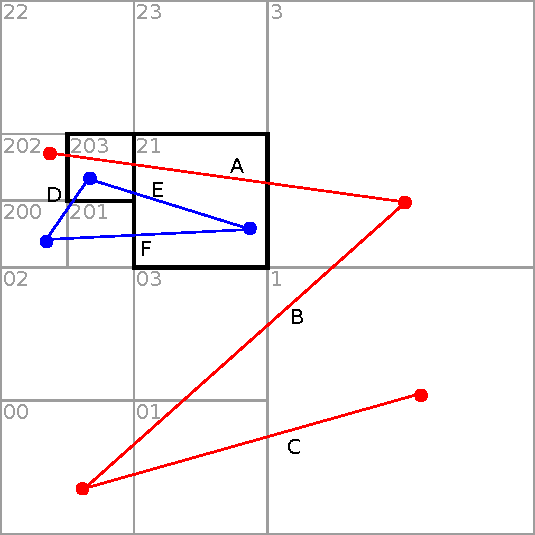
\includegraphics[width=0.48\columnwidth]{octree-cartesian-1.pdf} }
  \subfloat[][]{
    \label{fig:octree-hierarchical-1}
    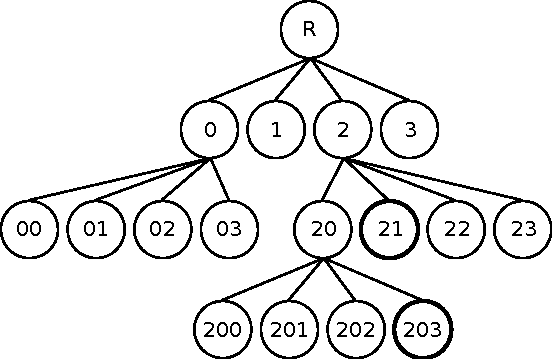
\includegraphics[width=0.48\columnwidth]{octree-hierarchical-1.pdf} } \\
  \subfloat[][]{
    \label{fig:octree-cartesian-2}
    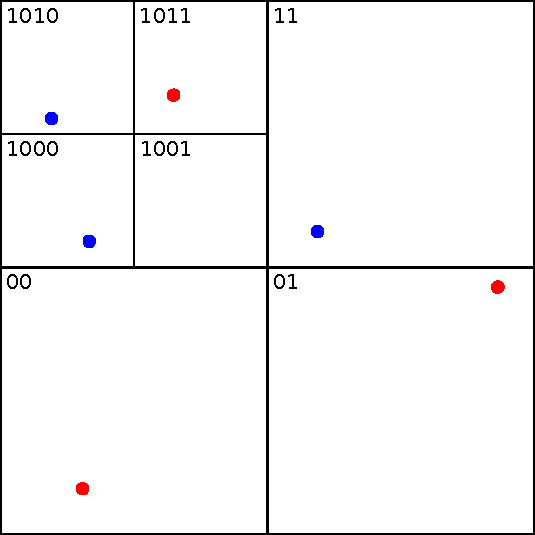
\includegraphics[width=0.48\columnwidth]{octree-cartesian-2.pdf} }
  \subfloat[][]{
    \label{fig:octree-hierarchical-2}
    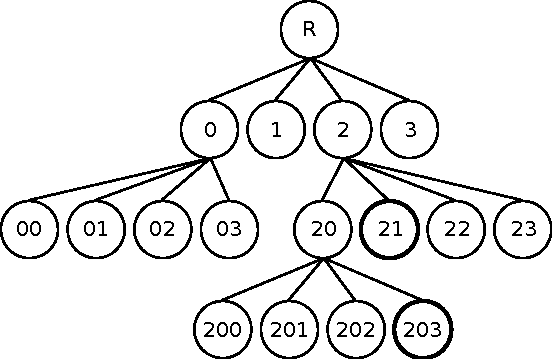
\includegraphics[width=0.48\columnwidth]{octree-hierarchical-2.pdf} }
  \caption{The $\container{l}{O}$ function finds the smallest octree cell that completely contains line $l$.
    \protect\subref{fig:octree-cartesian} Cartesian view of the octree with a red and a blue object.
    \protect\subref{fig:octree-hierarchical} Hierarchical view of the octree.
  }
  \label{fig:steps}
\end{figure}

In Fig. \ref{fig:steps}, R (Root) is the smallest containing cell for lines A, B, and C, cell 20 contains line D, and cell 2 contains lines E and F. After Step 3 of the algorithm, line A is stored in leaf cells 202, 203, 21, and 3. Conflict cells, which are the only cells that are subdivided, are 203 and 21.

%\begin{table}
%  \centering
%  \begin{tabular}{ll}
%    \toprule
%    line &  $\container{line}{O}$ \\
%    \midrule
%    A & R \\
%    B & R \\
%    C & R \\
%    D & 20 \\
%    E & 2 \\
%    F & 2 \\
%    \bottomrule
%  \end{tabular}
%\end{table}


%-----------------------------------------------------------
% Compute GVD surface
%-----------------------------------------------------------
\section{Compute GVD surface}
\label{sec:bisector}

%-------------------------------------------------------------------------------
% Results
%-------------------------------------------------------------------------------
\section{Results and applications}
Our implementation\footnote{Source code is available at \url{http://cedmav.org/research/project/33-gvds.html}.} of the algorithm supports \red{polygons and} triangulated objects, and our wavefront initialization step is implemented on the GPU using OpenCL. All tests were run on a MacBook Pro laptop with a dual-core 2.9 GHz processor, 8 GB memory, and Intel HD 4000 graphics card. Figure \ref{fig:bunny} shows our implementation of the GVD computation pipeline, and Figure \ref{fig:pipes} shows the computed GVD on a more challenging dataset.  We compare our method with other work and then show examples in three application settings: path planning, proximity queries, and exploded diagrams.

\subsection{Comparison to other methods}


% # octree vertices
%  52K ./viewer3 -l 8 ~/data/gears/gear[1-3].obj
% 170K ./viewer3 -l 12 ~/data/knife/knife-holder.obj ~/data/knife/knife[2-4].obj
% 146K ./viewer2 -l 24 ../data2/filled_ut/*.dat
% 2.8M ./viewer3 --uniform-colors -a 1 -l 8 ~/data/neuron/improved/a*.obj
% 1.3M ./viewer3 -l 8 ~/data/rice-dwarf/decimated2/n1UF2a-*.obj

% memory (54 bytes per octree cell)
%  2.8Mb ./viewer3 -l 8 ~/data/gears/gear[1-3].obj
%  9.2Mb ./viewer3 -l 12 ~/data/knife/knife-holder.obj ~/data/knife/knife[2-4].obj
% 7.9Mb ./viewer2 -l 24 ../data2/filled_ut/*.dat
% 151.2Mb ./viewer3 --uniform-colors -a 1 -l 8 ~/data/neuron/improved/a*.obj
% 70.2Mb ./viewer3 -l 8 ~/data/rice-dwarf/decimated2/n1UF2a-*.obj

\begin{table*}
  \centering
  \footnotesize{
  \begin{tabular}{l c c c c c c c}
    \toprule
    dataset & objects & object          & octree   & octree          & octree &
    GVD   & GVD             \\
            &         & $\Delta$s       & depth    & cells           & memory &
    (sec) & $\Delta$s       \\
            &         & ($\times 10^3$) &          & ($\times 10^3$) & (Mb)   &
          & ($\times 10^3$) \\
    \midrule
    % ./viewer3 -l 8 ~/data/gears/gear[1-3].obj
    Fig. \ref{fig:gears} & 3 & 7 & 8 & 54 & 3 & 0.9 & 83\\
    % ./viewer3 -l 12 ~/data/knife/knife-holder.obj ~/data/knife/knife[2-4].obj
    Fig. \ref{fig:knife} & 4 & 15 & 12 & 146 & 9 & 3.9 & 232 \\
    % ./viewer2 -l 24 ../data2/filled_ut/*.dat
    Fig. \ref{fig:path} & 470 & 5 & 24 & 158 & 8 & 2.0 & 151 \\
    % ./viewer3 --uniform-colors -a 1 -l 8 ~/data/neuron/improved/a*.obj
    Fig. \ref{fig:axons} & 448 & 4015 & 8 & 2716 & 151 & 195 & 8100 \\
    % ./viewer3 -l 8 ~/data/rice-dwarf/decimated2/n1UF2a-*.obj
    Fig. \ref{fig:mol-explode} & 35 & 1500 & 8 & 496 & 70 & 19 & 2700 \\
    \bottomrule
  \end{tabular}}
  \caption{Table of octree/GVD computation statistics and timings on datasets that are unmanageable using other methods. \red{Columns are: \emph{objects} - the number of objects in the dataset; \emph{object $\Delta$s} - the number of line segments (2D) or triangles (3D) of all objects in the dataset; \emph{octree depth} - required octree depth in order to resolve objects; \emph{octree cells} - total number of leaf octree cells; \emph{octree memory} - amount of memory used by the octree; \emph{GVD (sec)} - seconds to perform all steps of GVD computation; \emph{GVD $\Delta$s} - number of line segments (2D) or triangles (3D) in the GVD.}}
  \label{tab:timings}
\end{table*}


%-------------------------------------------------------------------------------
% Conclusions
%-------------------------------------------------------------------------------
\section{Conclusions}

%-------------------------------------------------------------------------------
% Acknowledgements
%-------------------------------------------------------------------------------
%\section*{Acknowledgements}
%Thanks to Kristen Harris for use of the neuronal data and Jonathan Bronson for the heart data. The work of JE and VP was supported in part by NSF IIS-1314896, NSF ACI-0904631, DOE/NEUP 120341, DOE/UV-CDAT DESC0006872, DOE/Codesign P01180734, DOE/SciDAC DESC0007446, DOE/PIPER DESC0010498, and DOE/CCMSC DENA0002375. This work initiated at the University of Texas when JE, ED  and CB were supported in part by NIH contract R01-EB00487, NSF Grant OCI-1216701 and SNL contract 1439100.

%-------------------------------------------------------------------------
% Bibliography
%-------------------------------------------------------------------------

%\bibliographystyle{eg-alpha}
\bibliographystyle{eg-alpha-doi}
\balance
\bibliography{paper}

\end{document}
